\begin{answer}
    Starting with $k=1$ the fitted curve looks very simple (high bias, low variance), and is just a line. The higher $k$ gets the higher the polynomial of the resulting fitted curve is, and the better it can try to approximate the data points.

    From $k > 5$ on (the point where also the features $\&$ degree of polynomial $>$ than the data points), we can see that the curves just get more complex without any real improvement, and seemingly irrelevant areas seem to get more complex. The curves start to overfit (high variance, low bias)
    \begin{figure}[h]
        \centering
        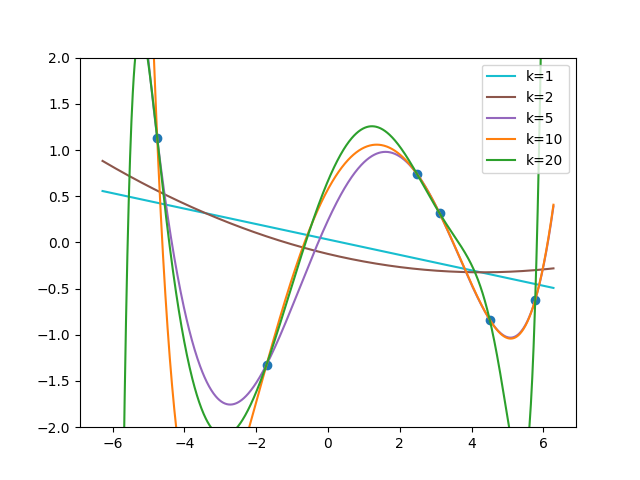
\includegraphics[width=0.8\textwidth]{src/featuremaps/plot-small-degrees[1, 2, 5, 10, 20].png}
        \caption{Polynomial regression with sine features}
        \label{fig:sine-features}
    \end{figure}
\end{answer}
